\documentclass[a4paper,10pt]{article}

\usepackage[utf8]{inputenc}
\usepackage{graphicx}           %package to display pics
\usepackage[section]{}  %to prevent pictures from floating around
\usepackage{float}


\title{\vspace{-10ex}A Smartphone Application For Home-based Hand Rehabilitation}
\author{Kody Fitch, Brandon Shepard, Martin Soto, Joseph Yang\and Supervisor: Professor Rahman}
\date{CS595 Spring 2019}

\begin{document}

\maketitle

\section{Abstract}
    Our goal is to design and prototype a smartphone based, hand rehabilitation application. Deliverable at the end of the project will be a fully functional smartphone application that guides and measures rehabilitation through the use of a wearable robotic glove. 

\section{Functionality}
    The smartphone application will communicate wirelessly with the robotic glove. The robotic glove will receive exercise direction from the application while communicating glove positional data back to the application. The application will process, display and communicate this glove data to the patient while simultaneously uploading hand data to the cloud. With the data stored in the cloud, the rehab professional can login to the application, access patient data and prescribe exercises remotely.
    \begin{figure}[h]
         \centering
         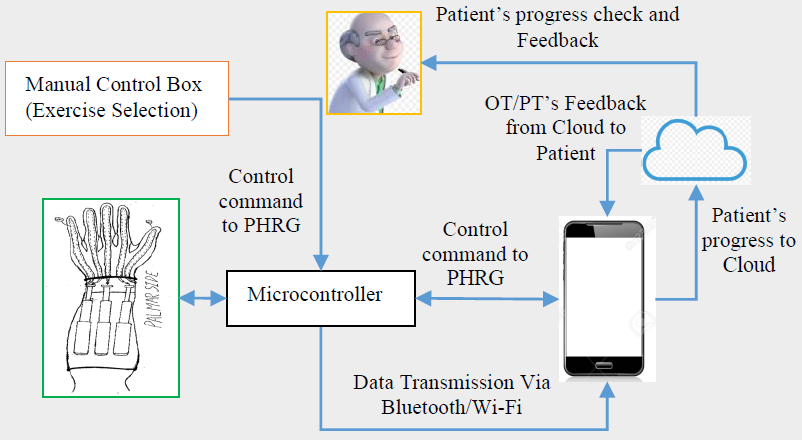
\includegraphics[width=1\textwidth]{rahmanSchematic}
         \caption{Rehabilitation System Schematic}
    \end{figure}
The long-term goals of the project is to have multiple physical augmentations so that different body parts can be rehabilitated through this application. In addition, in order to reduce workload from physicians and doctors, machine learning can be implemented to analyze the data generated in order to give advice to patients.

\section{Semester Scope}
Given the time and resource constraints for the capstone, the scope of the project has been scaled down as shown in figure 2.
	\begin{figure}[h]
		\centering
		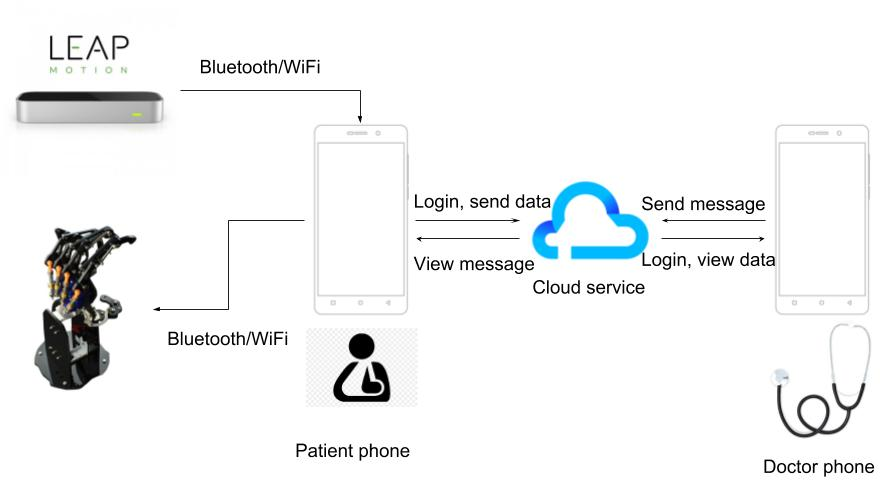
\includegraphics[width=1\textwidth]{semesterScope}
		\caption{Updated Project Scope}
	\end{figure}
The main change is the removal of the robotic glove. The glove has not been produced yet, so the project will use a Leap Motion device and robotic hand in its place. The Leap Motion device will reflect the motion tracking functionality of the glove and the robotic hand will reflect the assistive motion of the glove. By doind this, an API and communication protocol can be developed in lieu of the robotic glove. The glove can then be produced with the protocol and API in mind, allowing for straightforward replacement of the Leap Motion device and robotic hand when completed.

\section{Technologies}

    \subsection{Smartphone platform}
        We have chosen to use Ionic. Ionic is a framework based off the popular Angular platform created by Google. Ionic allows for the creation of platform agnosic, hybrid applications. A hybrid application supports both web applications and native applications, making it a strong choice for this project. Additionally, the ionic website appears to be well documentated and the platform comes with the majority of the components needed to complete the project.
        
    \subsection{Robotic glove simulation}
        A robotic glove prototype is being developed by Prof. Rahman's team at the UWM Biorobotics lab. In the mean time we will be simulating the glove with the use of Leap Motion sensor and a bionic robotic hand. Both items are being provided by the UWM Biorobtics lab.
        \begin{figure}[h]
         \centering
         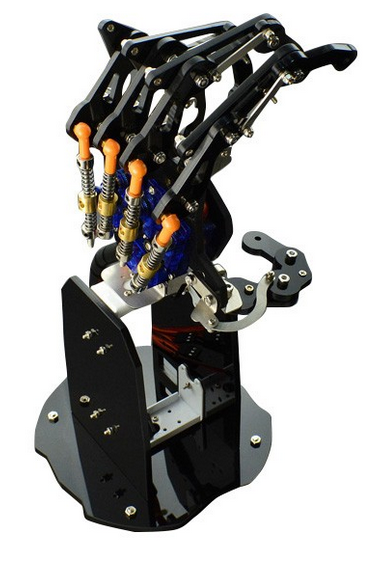
\includegraphics[width=50mm, scale=0.1]{bionicRoboticHand}
         \caption{Bionic Robotic Hand}
        \end{figure}
        
    \subsection{Cloud service}
        Amazon AWS will be used for our cloud service. The Ionic team and the Amazon AWS team seem to have a good relationship with each other and have collaborated in the past to make ionic applications easier to integrate with Amazon AWS. Furthermore since Amazon AWS is one of the most popular cloud platforms there is a lot of good documentation for it. 
        
    \subsection{Justification for \& alternative technologies}
        Project requirements and resource restrictions influence the platform to develop the phone application on. Native apps have better performance and more direct API to the phone's hardware, but require a seperate codebase for iOS and Android. Hybrid apps are great for rapid app development, but come with slower performance. The requirements do not require high performance such as 3D rendering and the app needd to be completed in a short amount of time, so the team has decided to use a hybrid platform.

        As with most web dev projects, there are countless alternatives. Some popular alternatives to Ionic include React Native (React), Kendo UI (JQuery) or Quasar (Vue). The platform decision was based on three criterion: 
        \begin{itemize}
         \item group skillset
         \item quality of documentation
         \item platform coverage
        \end{itemize}
        With quality of documentation and platform coverage being sufficient across the various platforms, the differentiator was group skillset. Overall, our group had the most experience with Angular platforms. As such, Ionic was decided upon.
        
        The robotic glove is currently in development, and there does not appear to be a marketed alternative. There appear to be alternatives to leap motion sensors, but since Prof. Rahman has provided and recommended the simulation hardware. As a result, we did not extensively search for alternatives. 
        
        In regards to the bionic hand. Generally speaking, as robotic hand precision increases so does cost. The main purpose of the hand is to confirm communication and sending locomotion instructions. It is a temporary device to be used until the glove is ready to replace it, so high precision is not required.  Again, Prof. Rahman has lead the decision process for robotic hand selection as he balances budgetary constraints with precision constraints. The product that was ordered is a \$219 hand from robotshop.com that is compatible with Arduino.

\section{Design}

        \subsection{Leap Motion to Robotic Hand}
            Since the Leap Motion device is a temporary device for prototyping, the goal is to convert the information from the Leap Motion into a format that is more universal. Two issues to solve with the Leap Motion device is that it produces data in their own structures and that the rate is too fast for the Arduino at 200 per second.
            \begin{figure}[h]
            \centering
            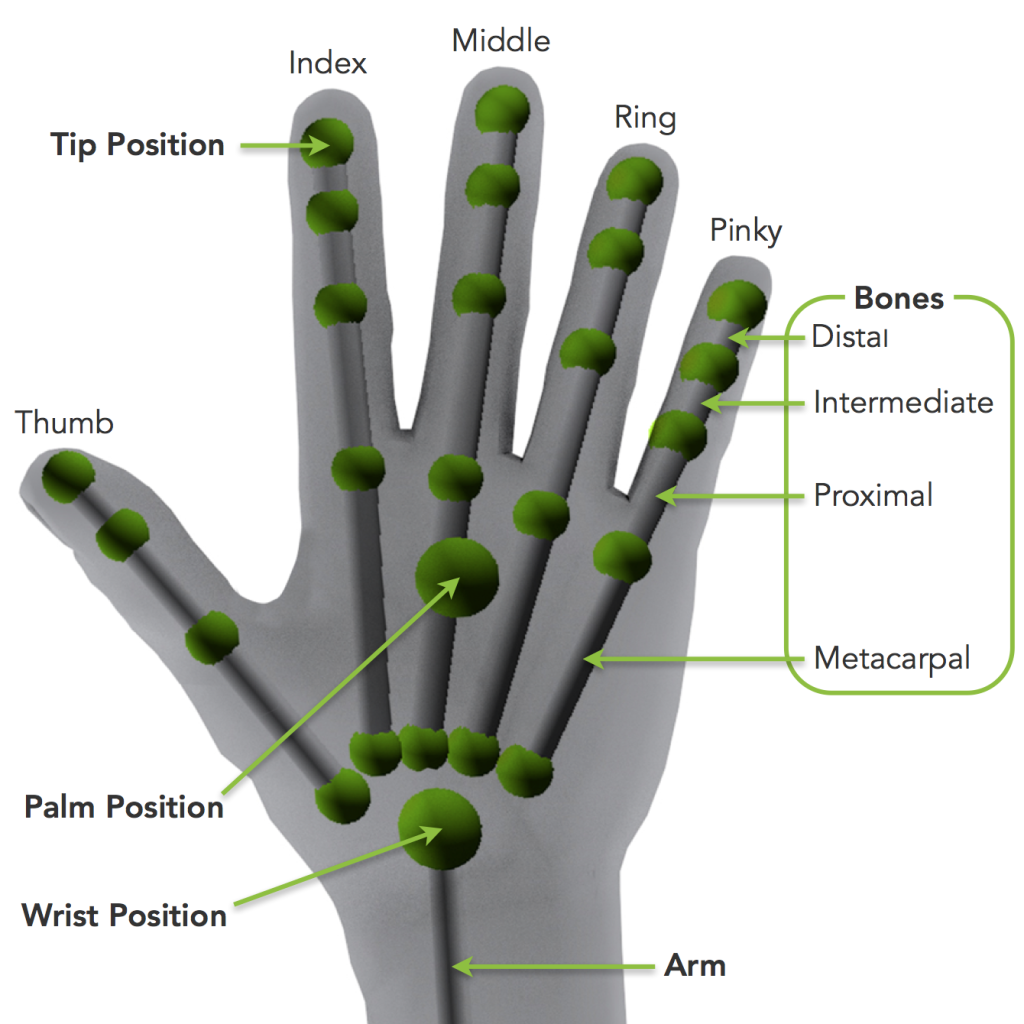
\includegraphics[width=90mm, scale=0.2]{hand-hierarchy-1024x1024}
            \caption{Leap Motion Frame Data}
            \end{figure}

            Figure 4  shows that data generated by the Leap Motion device while it tracks the hand. The information needed for the project is the angles of the fingers with respect to the palm. To get this information, the vector of the distal bone for each finger is gathered along with the vector for the normal of the palm. By doing a dot product between the distal vector and the palm vector, the angle between the two can be determined.
            \begin{figure}[h]
            \centering
            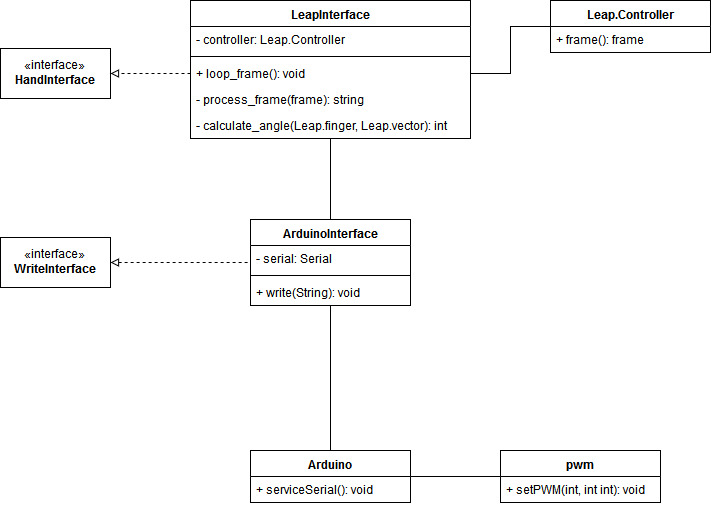
\includegraphics[width=140mm, scale=1]{LeapMotionArduinoERD}
            \caption{Leap Motion to Arduino}
            \end{figure}

            Figure 5 shows the general design of how data is extracted from the Leap Motion device and process by the Arduino. The data shown in Figure 4 comes in the form of frames via the LeapController. To deal with the 200 frames per second issue mention earlier, LeapInterface runs a a method, loop\_frame, that manually polls the LeapController at a reduced rate of 20 frames per second. The frames are then processed as described earlier and passed to the ArduinoInterface.The final string passed to the ArduinoInterface is in the form of a letter deliminated string, with each succeeding letter indicating the next finger. For example, if all the fingers were at 180 degrees, the string generated would be in the form "180a180b180c180d180e".

            The ArduinoInterface opens a serial connection to the Arduino and writes the string given to it. In the Arduino, while the serial buffer has information, serviceSerial builds an integer object and sends out the built integer as soon as it encounters an alphabetical character in the buffer. The Arduino is wired to the robotic hand's servos, with one servo for each finger. The servos take instructions in the form of pulse-width modulation (pwm), so another conversion needs to be made. Each servo has different tolerances, so minimum and maxisum pwm values are calibrated for each finger. For example, the thumb may have a minimum pwm of 200 and a maximum pwm of 400. serviceSerial maps the instruction, "180a", to those values and sends the value "400" to the pwm library for the thumb.
            
        \subsection{Ionic Application}
            The ionic application will be the main user interface for both the doctor and patient screens. The goal is to dynamically render all screens from the server metadata. This will be accomplished through a multi layered metadata schema and recursive programming. The benefits of this design choice include code reusability due to generic classes and a more maintainable code base. 
            
            The general flow of events within the ionic application begins with the user login screen. This screen will prompt the user for their login and password. If an account needs to be created the user can click the register button to create an account. After authentication, the user will enter the menu screen. If there is only a single patient, then only the patient's name will show up as a menu option. If the user is a doctor then a list of all patients will populate on the menu screen. After selecting a patient name from the menu screen, the user will be prompted with a second menu option: exercise, history, or advice. The exercise screen is how the doctor or patient can prescribe or rehab glove exercise modules. The history screen is where previous activity will be displayed, allowing the user to gauge progress. The advice screen is currently undefined, but it is expected to either display advice from the doctor and/or basic troubleshooting help.
            \begin{figure}[h]
            \centering
            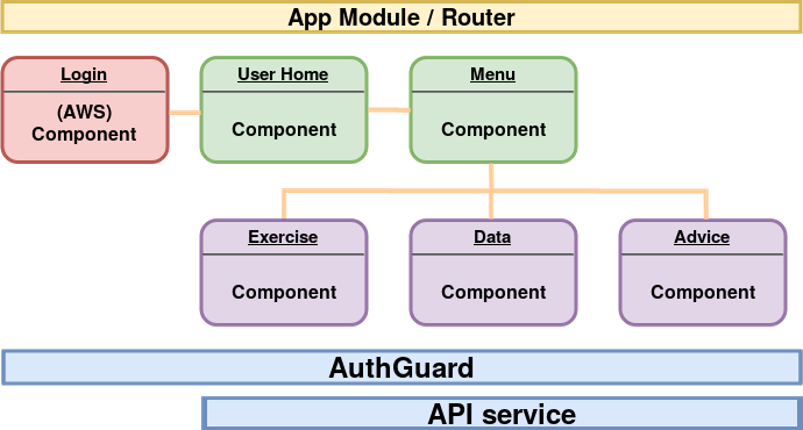
\includegraphics[width=140mm, scale=1]{ionicAppLayout}
            \caption{Ionic application diagram}
            \end{figure}
            
            Additional design decision include using an AuthGuard service to protect the logged in screens and a single app module. The AuthGuard functions in conjunction with an authentication service, which manages the storage of our session token. The current plan is to stick with one app module since the application only has a few screens right now. This decision may be revisited as the application grows in size (IE: it may make more sense to create additional modules to help structure a growing code base). 
            
        \subsection{Cloud Service}
	As mentioned before we will be using Amazon Cognito which will take care of all of our sign up, sign in, authentication, and forgot password services for users. All of the code is handled on the AWS side, we just simply display a module object on our html page. It has a built in UI which takes care of our login and sign up page design.

	The two AWS databases that are currently being decided on are Amazon DynamoDB and MySQL which can be used with Amazon. Amazon DynamoDB can potentially be used to retrieve the data for a user such as the exercises the user needs to do, or advice that was given by the doctor. The doctor advice data or exercise data that should be given to each user can be saved using this database. However, since DynamoDB is not a relational database, a MySQL database can potentially be used to hold the data and the relationships shown by the diagram down below.
	
	To work with the databases, we will be using two AWS services. We will be using Amazon API Gateway and AWS Lambda to create an API that can allows us to make CRUD (create/read/update/delete) operations with our database. AWS Lambda is a service that allows us to run code without needing a server. Amazon API Gateway is a service that allows us to make API's that can talk with our backend services. How it will work is that AWS will have the backend API in the AWS Lambda so that our mobile app can update or retrieve data when it needs it for our user at any time. In our code we will have functions that use the API endpoints to talk to the database when we need to save or update user or doctor information. 

            
            The design goal for the database was to avoid data redundancy and structure for simple lookups. In our design we will be using 5 tables: PATIENT, DOCTOR, EXERCISE, PRESCRIPTION, and RECORD. The RECORD table will be used primarily for the history screen. The PRESCRIPTION table will be the main stay for the exercise screen. We may need to add a connection between the DOCTOR and PATIENT tables to help support the main menu screen, but this is undecided currently. 
            
            \begin{figure}[H]
            \centering
            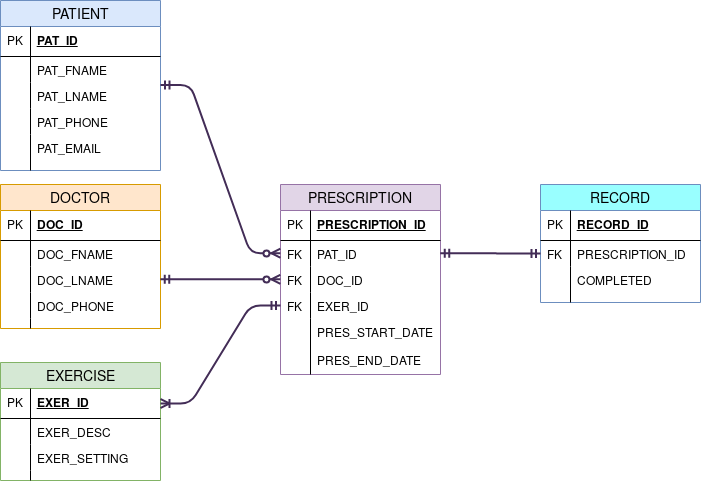
\includegraphics[width=140mm, scale=1]{databaseDiagram}
            \caption{Database ERD Diagram}
            \end{figure}
            

\section{Implementation}

            Each member has been assigned to a part of the project to be the resident expert in. The assignment is as follows:
        \begin{itemize}
         \item Kody Fitch: Leap Motion
         \item Brandon Shepard: Ionic Application
         \item Martin Soto: AWS Cloud
         \item Joseph Yang: Mechanical Hand
        \end{itemize}

            Progress is tracked through milestones in implementation. The first milestone is to establish a serial connection from the Leap Motion device to the mechanical hand and to control the hand through data gathered from the Leap Motion device. The following milestone is to include the Ionic application through a bluetooth connection. The Ionic application would act as a router for data between the Leap Motion device and the mechanical hand. Finally would be to connect the AWS cloud to the application.

            When the process flow is complete with all platforms connected, features will be added as time allows. These features include messaging between doctors and patients, voice control, and unique interfaces for doctors and patients.

\section{Conclusion}

          In conclusion, the project is to design and produce a prototype for a smartphone based, hand rehabilitation application. This project has many different platforms that need to be connected to each other including the Leap Motion device, Arduino, mechanical hand, Ionic, and AWS. Since the long term goal is to allow for different types of rehabilitation devices to be used, care has been taken for the design of the interfaces between the platforms.

\end{document}
